\documentclass{article}
\usepackage{../report}
\graphicspath{ {./imgs} }
\title{Lab 9 Report}

\begin{document}
\maketitle
\section{Introduction}
In this lab we are studying the DC biasing of an NPN
transistor. Refer to Figure \ref{fig:maincircuit} to 
see the circuit that we are building today. Via analysis
of the circuit we will select resistor values that
allow us to force this transistor to operate in the
active and saturation regions.

\begin{figure}[!h]
  \begin{center}
  \begin{circuitikz}[american]
    % \ctikzset{tripoles/mos style/arrows}
    \ctikzset{}
    \draw (0,-3) node[vee](Vee){}
    to[resistor, l=R$_2$] (0,0)
    to[resistor, l=R$_1$] (0,3) node[vcc](Vcc){};
    \draw (0,0) -- (1,0) node[npn, anchor=B](Q){};
    \draw (Q.C) to[resistor, l_=R$_C$] (Q.C |- Vcc) node[vcc]{};
    \draw (Q.E) to[resistor, l=R$_E$] (Q.E |- Vee) node[vee]{};
    % \node[below=7.5mm, right=-1mm] at (Vee) {$V_{EE}=\SI{-10}{V}$};
    \node[below=7.5mm, right=9mm, anchor=center] at (Vee) {$V_{EE}=\SI{-15}{V}$};
    \node[above=7.5mm, right=9mm, anchor=center] at (Vcc) {$V_{CC}=\SI{15}{V}$};
    \node[above=4mm] at (Q.B) {B};
    \node[right=3mm] at (Q.C) {C};
    \node[right=3mm] at (Q.E) {E};
  \end{circuitikz}
  \caption{NPN Transistor Circuit}
  \label{fig:maincircuit}
  \end{center}
\end{figure}

\section{Active Region}
We are tasked to design the circuit such that
it follows the requirements shown in Figure
\ref{table:activeTable}.

\begin{figure}[h!]
\begin{center}
  \begin{tabular}{r|l}
    I$_C$ & $\SI{1}{mA}$ \\
    V$_B$ & $\SI{0}{V}$ \\
    V$_C$ & $\SI{5}{V}$ 
  \end{tabular}
\end{center}
\caption{Table showing required values for NPN transistor
in the Active Region.}
\label{table:activeTable}
\end{figure}

\subsection{Hand Calculations}

Using the value for $\beta$ that we got in the last lab
($\beta=161.02$) we are able to determine the relationships
between some currents through the transistor. We found
$i_B$ by using the equation $i_B=\frac{i_C}{\beta}=\SI{6.21}{\mu A}$.
These leaves the equation $i_E=i_C + i_B$. $i_E=\SI{1.00621}{mA}$.

We now have enough information to determine the values
of R$_C$ and R$_E$. Using Ohm's Law over the resistors,
and knowing that the values of V$_C$ and V$_E$ are
5 V and $-0.7$ V respectively, we could calculate the
resistor values. R$_C=\SI{10}{k \Omega}$ and R$_E=\SI{14.211}{k
\Omega}$.  I used a script that I wrote to find resistors
values that are within 1 percent of the required values
using a combination of resistors available in the lab.

After an analysis of the left side of the circuit,
we can find the resistor values that allow close to
$\SI{6.21}{\mu A}$ of current to flow through the base
terminal of the transistor.  We selected a resistor
R$_1$ that allows a current about 200 times the size
of the base current through R$_1$.  The selected resistor
value was $\SI{12.077}{k \Omega}$, and this was done
so that small variations in the current through R$_1$
will still result in enough current to flow through
the base of the transistor.

Using KCL and some algebra we are able to find an
expression for R$_2$ in terms in R$_1$. 
$$R_2=\frac{\SI{15}{V} R_1}{\SI{15}{V} - \SI{6.21}{\mu A} R_1}$$

Using our selected value for R$_1$ we can find a value
for R$_2$.  We selected R$_2=\SI{12.138}{k \Omega}$.
Because the values for R$_1$ and R$_2$ are very close
together (within the tolerance of the resistors available
to us in the lab), controlling the amount of current
going through the base will be difficult, and we can
basically achieve the same result by selecting identical
resistors within the same order of magnitude. Because
of that we selected a resistor value of $\SI{15}{k \Omega}$
because there were plenty available in our lab.

\subsection{Multisim Analysis}

With all of those values selected we were able to build
our circuit and analyze it. First we built the circuit in
Multisim and did a digital analysis of the circuit to
check the voltages and verify that the circuit was 
operating in the Active region. You can see that simulation
in Figure \ref{fig:multisimPart1}.

\begin{figure}[h!]
  \begin{center}
  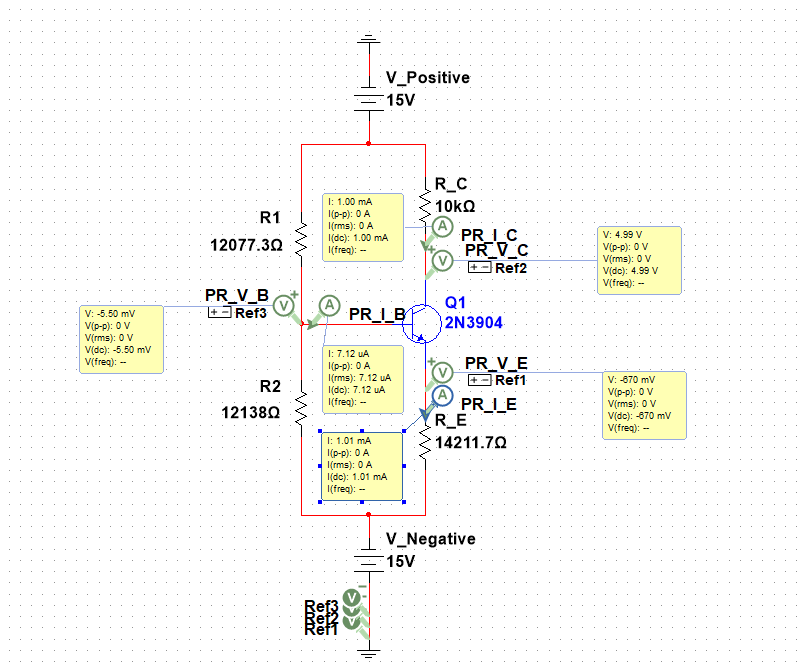
\includegraphics[width=0.6\textwidth]{Multisim Simulation Image.png}
  \caption{Multisim Simulation for NPN transistor
  in the Active Region}
  \label{fig:multisimPart1}
  \end{center}
\end{figure}

In the simulation results you can see that the voltages
and currents are in line with our calculations.
Notably: V$_E=\SI{-0.67}{V}$ and V$_B=\SI{-0.006}{V}$,
which are within tolerance to be the values that
we calculated. Figure \ref{table:activeTableSim} is
a table enclosing all of our values that we simulated.

\begin{figure}
  \begin{center}
    \begin{tabular}{r|r}
      V$_C$ & $\SI{4.99}{V}$ \\
      V$_E$ & $\SI{-0.67}{V}$ \\
      V$_B$ & $\SI{-5.5}{mV}$ \\
      I$_C$ & $\SI{1.00}{mA}$ \\
      I$_E$ & $\SI{1.01}{mA}$ \\
      I$_B$ & $\SI{7.12}{\mu A}$ \\

    \end{tabular}
  \end{center}
  \caption{Table of Multisim simulated values}
  \label{table:activeTableSim}
\end{figure}

\subsection{Prototyping and Measurement}

Using the earlier noted resistor values and a transistor
we built the circuit and made measurements of our own
to analyze the behavior of an NPN transistor in the
Active Region. Figure \ref{table:activeTableMeas} shows
the values that we measured from the physical circuit.

\begin{figure}[h!]
  \begin{center}
    \begin{tabular}{r|r}
      V$_C$ & $\SI{5.308}{V}$ \\
      V$_E$ & $\SI{-0.713}{V}$ \\
      V$_B$ & $\SI{-52.4}{mV}$ \\

    \end{tabular}
  \end{center}
  \caption{Table of measured voltages}
  \label{table:activeTableMeas}
\end{figure}

These values are well in line with the calculated values
considering the variations in transistors and resistor
values.

\subsection{Post-Measurement Exercise}

V$_{BE}$ resulted in a value of $\SI{0.66}{V}$.
V$_{CE}$ resulted in a value of $\SI{6.021}{V}$.
These values are close to our calculated values,
V$_C$ was a little high which resulted in a skewed
V$_{CE}$ as well, but both still suggest operation in
the Active Region.

Using our measured resistor values we found 
the following currents shown in Figure
\ref{table:activeTableMeasCurrent}.

\begin{figure}[h!]
  \begin{center}
    \begin{tabular}{r|r}
      I$_C$ & $\SI{1.003}{mA}$ \\
      I$_E$ & $\SI{0.998}{mA}$ \\
      I$_B$ & $\SI{-0.005}{mA}$ \\

    \end{tabular}
  \end{center}
  \caption{Table of measured currents}
  \label{table:activeTableMeasCurrent}
\end{figure}

From the measured currents we can see that the base
current is in the wrong direction, but that can
be concluded from the tolerance of the resistors. It
still operates in the active region regardless.

% 
% 
\newpage
% 
% 
% 

\section{Saturation Region}
We are tasked to design the circuit such that
it follows the requirements shown in Figure
\ref{table:satTable}.

\begin{figure}[h!]
\begin{center}
  \begin{tabular}{r|l}
    I$_C$ & $\SI{1}{mA}$ \\
    I$_E$ & $\SI{1.2}{mA}$ \\
    V$_C$ & $\SI{2}{V}$ \\
    V$_{CE}$ & $\SI{0.2}{V}$ \\
  \end{tabular}
\end{center}
\caption{Table showing required values for NPN transistor
in the Saturation Region.}
\label{table:satTable}
\end{figure}

\subsection{Hand Calculations}

Knowing that the value of V$_{CE}$ is 0.2 V, the
value for V$_E$ is 1.8 V. Using the constant drop 
model for V$_{BE}=\SI{0.7}{V}$ we find that the
voltage of V$_B$ is 2.5 V. This allows us to calculate
the values of R$_C$ and R$_E$ because we know
the currents that have to flow through those resistors.

The values that we found for R$_C$ and R$_E$ were 
$\SI{13}{k \Omega}$ and $\SI{14}{k \Omega}$ respectively.
We once again used the script that I wrote to select
resistors networks to match those values.

We are able to find the forced $\beta$ that is being
used in this saturation region.
$\beta_{forced}=\frac{i_C}{i_B}=5$

We decided to leave R$_2$ open to allow all the current
to flow through R$_1$ and then through the base terminal
of the transistor. We selected R$_1=\SI{62.5}{k \Omega}$.
R$_2$ can be any very large resistor, but we just left
it open completely.


\subsection{Multisim Analysis}

With all of those values selected we were able to build
our circuit and analyze it. First we built the circuit in
Multisim and did a digital analysis of the circuit to
check the voltages and verify that the circuit was 
operating in the Saturation region. You can see that
simulation in Figure \ref{fig:multisimPart2}.

\begin{figure}[h!]
  \begin{center}
  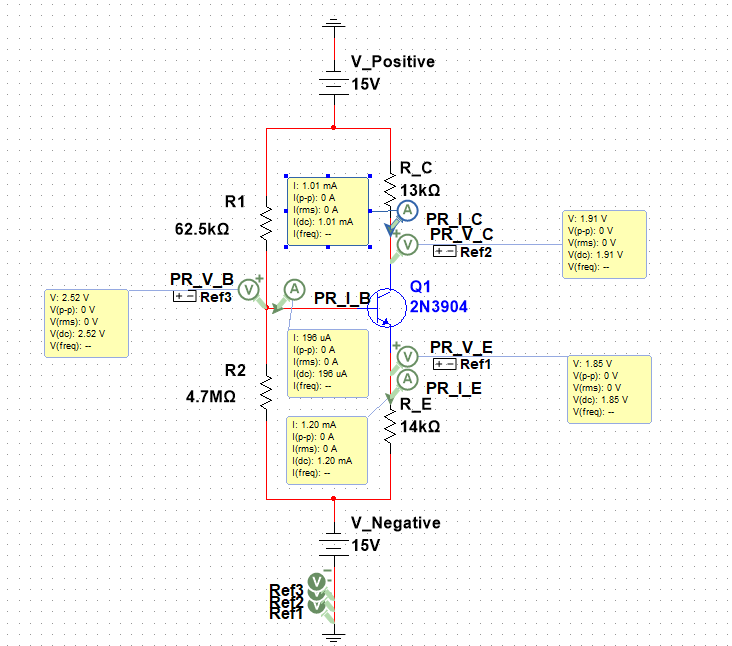
\includegraphics[width=0.6\textwidth]{Multisim Simulation Image Part 2.png}
  \caption{Multisim Simulation for NPN transistor
  in the Saturation Region}
  \label{fig:multisimPart2}
  \end{center}
\end{figure}

In the simulation results you can see that the voltages
and currents are in line with our calculations.
Figure \ref{table:satTableSim} is
a table enclosing all of our values that we simulated.

\begin{figure}
  \begin{center}
    \begin{tabular}{r|r}
      V$_C$ & $\SI{1.91}{V}$ \\
      V$_E$ & $\SI{1.85}{V}$ \\
      V$_B$ & $\SI{2.52}{mV}$ \\
      I$_C$ & $\SI{1.01}{mA}$ \\
      I$_E$ & $\SI{1.20}{mA}$ \\
      I$_B$ & $\SI{196}{\mu A}$ \\

    \end{tabular}
  \end{center}
  \caption{Table of Multisim simulated values}
  \label{table:satTableSim}
\end{figure}

Interestingly, V$_{CE}$ is just 0.06 V, but 
that still suggests that the transistor is
operating in the Saturation Region.

\subsection{Prototyping and Measurement}

Using the earlier noted resistor values and a transistor
we built the circuit and made measurements of our own
to analyze the behavior of an NPN transistor in the
Saturation Region. Figure \ref{table:satTableMeas} shows
the values that we measured from the physical circuit.

\begin{figure}[h!]
  \begin{center}
    \begin{tabular}{r|r}
      V$_C$ & $\SI{2.087}{V}$ \\
      V$_E$ & $\SI{2.040}{V}$ \\
      V$_B$ & $\SI{2.717}{mV}$ \\

    \end{tabular}
  \end{center}
  \caption{Table of measured voltages}
  \label{table:satTableMeas}
\end{figure}

Once again we see a smaller V$_{CE}$ than we would
expect, but that still suggests operation in 
the saturation region, and as you'll see the currents
are well in line with the requirements as well.

\subsection{Post-Measurement Exercise}

V$_{BE}$ resulted in a value of $\SI{0.677}{V}$.
V$_{CE}$ resulted in a value of $\SI{0.047}{V}$.

Using our measured resistor values we found 
the following currents shown in Figure
\ref{table:satTableMeasCurrent}.

\begin{figure}[h!]
  \begin{center}
    \begin{tabular}{r|r}
      I$_C$ & $\SI{0.993}{mA}$ \\
      I$_E$ & $\SI{1.19}{mA}$ \\
      I$_B$ & $\SI{0.197}{mA}$ \\

    \end{tabular}
  \end{center}
  \caption{Table of measured currents}
  \label{table:satTableMeasCurrent}
\end{figure}

The currents are right in line with the requirements
and the calculations completed earlier.

This also leaves a $\beta_{forced}=5.038$ which is 
right on top of the calculated value of $\beta_{forced}=5$
from the hand calculations.

\end{document}